\documentclass{standalone}
\usepackage{graphicx}	
\usepackage{amssymb, amsmath, amsthm}
\usepackage{color}

\usepackage{tikz}
\usetikzlibrary{arrows.meta, math, shapes}

\definecolor{light}{RGB}{220, 188, 188}
\definecolor{mid}{RGB}{185, 124, 124}
\definecolor{dark}{RGB}{143, 39, 39}
\definecolor{highlight}{RGB}{180, 31, 180}
\definecolor{lightteal}{RGB}{107, 142, 142}
\definecolor{midteal}{RGB}{72, 117, 117}
\definecolor{darkteal}{RGB}{29, 79, 79}
\definecolor{gray10}{gray}{0.1}
\definecolor{gray20}{gray}{0.2}
\definecolor{gray30}{gray}{0.3}
\definecolor{gray40}{gray}{0.4}
\definecolor{gray60}{gray}{0.6}
\definecolor{gray70}{gray}{0.7}
\definecolor{gray80}{gray}{0.8}
\definecolor{gray90}{gray}{0.9}
\definecolor{gray95}{gray}{0.95}

\tikzmath{
  function xparabola(\y, \xv, \yv, \S) {
    return 0.5 * ( (\xv + \S) - (\y - \yv) * (\y - \yv) / (\S - \xv) );
  };
  function pairint(\xa, \ya, \xb, \yb, \S) {
    \a = \xb - \xa;
    \b = \yb * (\S - \xa) - \ya * (\S - \xb);
    \c = \yb * \yb * (\S - \xa) - \ya * \ya * (\S - \xb) - (\S - \xa) * (\S - \xb) * (\xb - \xa);
    \d = sqrt( \b * \b - \a * \c);
    \yint = (\b + \d) / \a;
    if \yint < \ya then {
      \yint = (\b - \d) / \a;
    };
    if \yint > \yb then {
      \yint = (\b - \d) / \a;
    };
    return \yint;
  };
}

\begin{document}

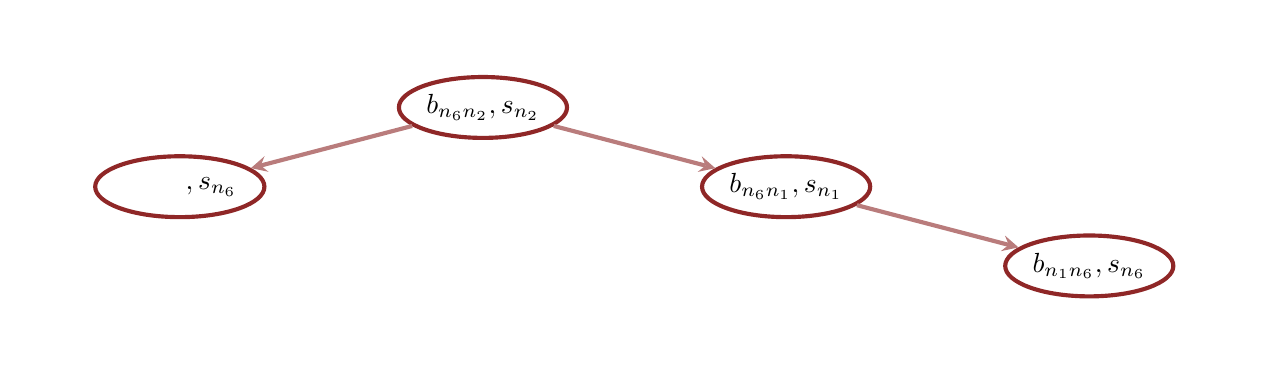
\begin{tikzpicture}[scale=0.35,
   obscirc/.style={circle, draw=dark, fill=dark, line width=1.5, text=white,
               inner sep=5, minimum size=27},
   obsell/.style={ellipse, draw=dark, fill=dark, line width=1.5, text=white,
                  inner sep=5, minimum height=27},
   unobscirc/.style={circle, draw=dark, fill=white, line width=1.5, text=black,
                     inner sep=5, minimum size=27},
   unobsell/.style={ellipse, draw=dark, fill=white, line width=1.5, text=black,
                    inner sep=1, minimum height=22}
  ]
  
  \begin{scope}[shift={(0, -11.5)}]
    \draw[white] (-7, -5) rectangle (44 - 7, 6.5);
  
    \node (N1) at (9.5, -5 + 3 * 2.875) [unobsell] { $b_{n_{6} n_{2}}, s_{n_{2}}$ };
    
    \node (N2) at (-1.5, -5 + 2 * 2.875) [unobsell] { $\hspace{8mm}, s_{n_{6}}$ };
    \node (N3) at (20.5, -5 + 2 * 2.875) [unobsell] { $b_{n_{6} n_{1}}, s_{n_{1}}$ };
    
    \node (N4) at (31.5, -5 + 2.875) [unobsell] { $b_{n_{1} n_{6}}, s_{n_{6}}$ };
  
  
    \foreach \B/\E in {N1/N2, N1/N3, N3/N4} {
      \draw[->, >=stealth, color=mid, line width=1.5] (\B) -- (\E);
    }
  
  \end{scope}

\end{tikzpicture}

\end{document}  